\documentclass[usenames, dvipsnames]{beamer}
\usetheme[progressbar=frametitle]{metropolis}
\usepackage[utf8]{inputenc}

\usepackage{amsmath}

\usepackage{amssymb}

\usepackage{amsfonts}

\usepackage{stmaryrd}

\usepackage{mdframed}

\usepackage{mathpartir}

\usepackage{xcolor}
\newcommand{\bluegreen}[1]{\textcolor{JungleGreen}{#1}}
\newcommand{\green}[1]{\textcolor{ForestGreen}{#1}}
\newcommand{\orange}[1]{\textcolor{BurntOrange}{#1}}
\newcommand{\blue}[1]{\textcolor{NavyBlue}{#1}}
\newcommand{\gray}[1]{\textcolor{gray}{#1}}
\newcommand{\mcolor}[2]{\color{#1}#2\color{black}}

\usepackage{lmodern}

\usepackage{pifont}

\usepackage{dedukti}
\usepackage{minted}
\usepackage{tikz}

\usetikzlibrary{arrows,shapes,decorations.pathmorphing,backgrounds,positioning,fit, calc}

\definecolor{blue-violet}{rgb}{0.54, 0.17, 0.89}

\usetheme{Montpellier}

\setbeamertemplate{headline}{}

\setbeamertemplate{background}{}


\newcommand{\cmark}{\textcolor{ForestGreen}{\ding{51}}}%
\newcommand{\xmark}{\textcolor{red}{\ding{55}}}%
\newcommand{\un}[1]{\textcolor{BrickRed}{#1}}
\newcommand{\transp}[2][30]{\color{fg!#1}#2\color{black}}
\newcommand{\defn}{:\equiv}

\newcommand{\Prop}{\textcolor{MidnightBlue}{\ensuremath{\mathbf{Prop}}}}

\newcommand{\Type}{\textcolor{Orchid}{\ensuremath{\mathbf{Type}}}}
\newcommand{\Typethree}{\textcolor{Orchid}{\ensuremath{\mathbf{Type}_3}}}
\newcommand{\Typefour}{\textcolor{Orchid}{\ensuremath{\mathbf{Type}_4}}}
\newcommand{\Kind}{\textcolor{RedViolet}{\ensuremath{\mathbf{Kind}}}}


\newcommand{\sttm}{STT\(\forall\)}

\newcommand{\qzero}{\ensuremath{\mathcal{Q}_0}}

\newcommand{\absT}[3]{\lambda#1^{#2}.~#3}

\newcommand{\forallT}[3]{\ensuremath{\forall #1^{#2}.~#3}}

\newcommand{\Rule}[2]{\inferrule*[right=#2]{ }{#1}}

\newcommand{\RuleP}[3]{\inferrule*[right=#3]{#1}{#2}}

\newcommand{\RulePP}[4]{\inferrule*[right=#4]{#1 \\ #2}{#3}}

\newcommand{\RulePPP}[5]{\inferrule*[right=#5]{#1 \\ #2 \\ #3}{#4}}

\newcommand{\addrule}[1]{#1 \and}

\newcommand{\subst}[3]{#1[#2\aff#3]}

\newcommand{\aff}{:=}

\newcommand{\forallp}[0]{\rotatebox[origin=c]{180}{\ensuremath{\mathcal{A}}}}

\newcommand{\forallP}[2]{\ensuremath{\forallp #1.~#2}}


\newcommand{\cicw}{\ensuremath{CiC\omega}}
\newcommand{\sttabd}{\ensuremath{STT\forall_{\beta\delta}}}

\newenvironment{rules}[2]
{
  \def\tmpvariable{#1}
  \label{#2}
  \begin{figure}
    \begin{mdframed}
  \begin{center}
  \begin{mathpar}
}
{
\end{mathpar}
\end{center}
\renewcommand{\figurename}{Fig.}
\caption{\tmpvariable}
\end{mdframed}
\end{figure}

}

\author{François Thiré}

\date{\today}

\title{(Proof) Interoperability between proof systems with the Logical Framework Dedukti}
\institute{Nomadic Labs}

\begin{document}

\maketitle

\section{Introduction}

\begin{frame}
  \begin{center}
    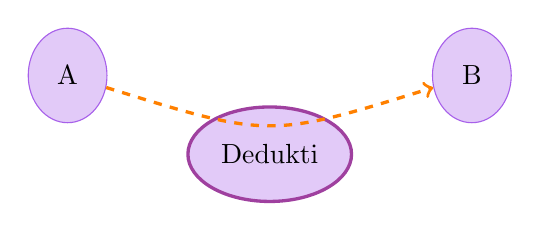
\begin{tikzpicture}[ checker/.style = {shape=ellipse,
        draw=blue-violet!75, fill=blue-violet!25, align=center,
        minimum height=1.2cm, minimum width=1cm}, checkers/.style =
      {shape=ellipse, draw=violet!75, very thick, fill=blue-violet!25,
        align=center, minimum height=1.2cm, minimum width=2cm},
      post/.style={->, >=stealth', semithick}]

      \node [checkers] (Dedukti) {Dedukti};
      \node [checker] (A) [left=of Dedukti,yshift=1cm] {A};
      \node [checker] (B) [right=of Dedukti, yshift=1cm] {B};
      \draw[very thick,dashed,->, orange] (A) .. controls ([yshift=0.2cm]Dedukti) .. (B);
    \end{tikzpicture}
  \end{center}
\end{frame}

\begin{frame}
  \begin{center}
    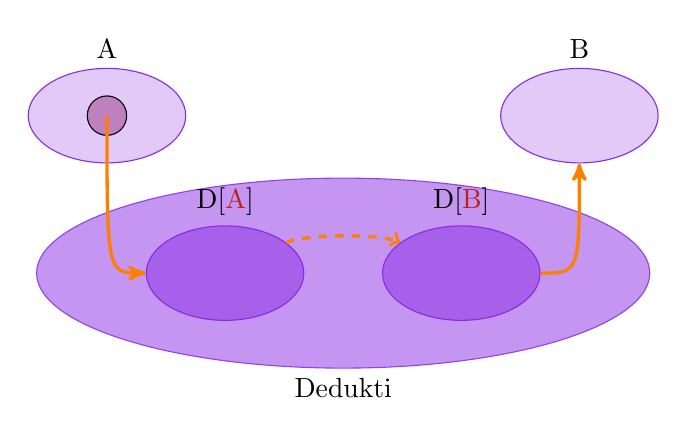
\begin{tikzpicture}
      [node distance=3cm, on grid, checker/.style = {shape=ellipse,
        draw=blue-violet!100, fill=blue-violet!25, align=center,
        minimum height=1.2cm, minimum width=2cm}, dedukti node/.style
      = {shape=ellipse, draw=blue-violet!90, fill=blue-violet!50,
        label={south:Dedukti}}, post/.style={->, >=stealth',
        semithick}]

      \node [checker, fill=blue-violet!75, label={north:D[\textcolor{BrickRed}{B}]}] (DB) {};
      \node [checker, left=of DB, fill=blue-violet!75, label={north:D[\textcolor{BrickRed}{A}]}] (DA) {};
      \begin{scope}[on background layer]
        \node [dedukti node, inner sep=7pt, fit={(DA) (DB)}]
        (Dedukti) {};
      \end{scope}
      \node [draw=none] (Coq) [above=of Dedukti] {};

      \node [checker, label={north:B}] (B) [right=of Coq,
      yshift=-1cm] {};

      \node [checker, label={north:A}] (A) [left=of Coq,
      yshift=-1cm] {};

      \draw[circle,fill=violet!50] (A.center) circle (0.25) {};

      \draw[post, very thick, ->, orange] (A.center) .. controls
      ([yshift=-0cm,xshift=-3cm]Dedukti) .. (DA); \draw[post,
      very thick, <-, orange] (B) .. controls
      ([yshift=-0cm,xshift=3cm]Dedukti) .. (DB);

      \draw[very thick, orange, dashed, ->] (DA) .. controls
      ([xshift=-0.5cm,yshift=0.5cm]Dedukti) and
      ([xshift=0.5cm,yshift=0.5cm]Dedukti) .. (DB);
    \end{tikzpicture}
  \end{center}
\end{frame}

\begin{frame}{The quadratic problem reloaded?}
  \begin{center}
    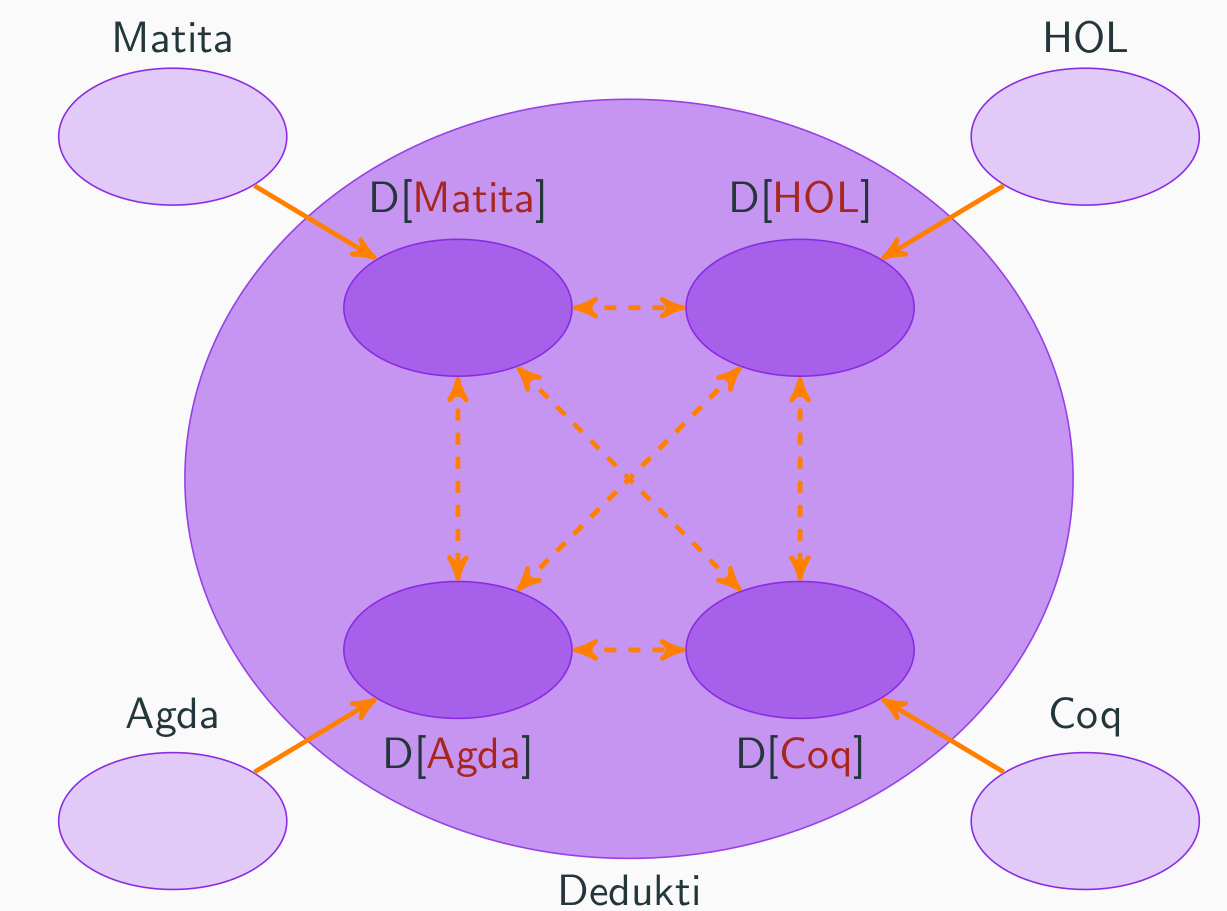
\includegraphics[scale=0.2]{images/quadratic.png}
  \end{center}
\end{frame}

\begin{frame}
  \begin{center}
    \Large{What are the advantages of using Dedukti for \orange{interoperability}?}
  \end{center}
  \pause
  \begin{center}    
    This is what we will try to \green{answer} during this lecture!
  \end{center}    
\end{frame}

\begin{frame}[fragile]{Setup for the demo}
  \begin{minted}{bash}
opam install dedukti
opam install universo
git clone https://github.com/Deducteam/Dedukti
git checkout francois@summer-school
cd Dedukti/summer-school
\end{minted}
\end{frame}

\begin{frame}{Objective of the demo}
  \begin{center}
    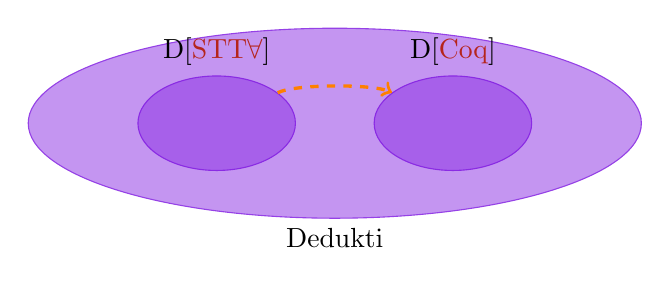
\begin{tikzpicture}
      [node distance=3cm, on grid, checker/.style = {shape=ellipse,
        draw=blue-violet!100, fill=blue-violet!25, align=center,
        minimum height=1.2cm, minimum width=2cm}, dedukti node/.style
      = {shape=ellipse, draw=blue-violet!90, fill=blue-violet!50,
        label={south:Dedukti}}, post/.style={->, >=stealth',
        semithick}]

      \node [checker, fill=blue-violet!75, label={north:D[\textcolor{BrickRed}{Coq}]}] (DB) {};
      \node [checker, left=of DB, fill=blue-violet!75, label={north:D[\textcolor{BrickRed}{STT\(\forall\)}]}] (DA) {};
      \begin{scope}[on background layer]
        \node [dedukti node, inner sep=7pt, fit={(DA) (DB)}]
        (Dedukti) {};
      \end{scope}
      % \node [draw=none] (Coq) [above=of Dedukti] {};

      % \node [checker, label={north:Coq}] (B) [right=of Coq,
      % yshift=-1cm] {};

      % \node [checker, label={north:STT\(\forall\)}] (A) [left=of Coq,
      % yshift=-1cm] {};

      % \draw[circle,fill=violet!50] (A.center) circle (0.25) {};

      % \draw[post, very thick, ->, orange] (A.center) .. controls
      % ([yshift=-0cm,xshift=-3cm]Dedukti) .. (DA); \draw[post,
      % very thick, <-, orange] (B) .. controls
      % ([yshift=-0cm,xshift=3cm]Dedukti) .. (DB);

      \draw[very thick, orange, dashed, ->] (DA) .. controls
      ([xshift=-0.5cm,yshift=0.5cm]Dedukti) and
      ([xshift=0.5cm,yshift=0.5cm]Dedukti) .. (DB);
    \end{tikzpicture}
  \end{center}
\end{frame}


\begin{frame}{The logical framework Dedukti}
    \begin{center}
      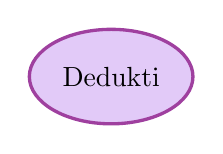
\begin{tikzpicture}[ checker/.style = {shape=ellipse,
          draw=blue-violet!75, fill=blue-violet!25, align=center,
          minimum height=1.2cm, minimum width=1cm}, checkers/.style =
        {shape=ellipse, draw=violet!75, very thick,
          fill=blue-violet!25, align=center, minimum height=1.2cm,
          minimum width=2cm}, post/.style={->, >=stealth', semithick}]

        \node [checkers] (Dedukti) {Dedukti};
      \end{tikzpicture}
    \end{center}

  \begin{center}
    Dedukti is a \orange{syntax} for \blue{dependent types} and \blue{rewriting}
  \end{center}
\end{frame}

\begin{frame}[fragile]{Dedukti syntax (1/2)}
  \begin{dedukti}
nat : Type.

0 : nat.

S : nat -> nat.

def plus : nat -> nat -> nat.

[m]   plus 0     m --> m.
[n,m] plus (S n) m --> S (plus n m).
\end{dedukti}
\end{frame}

\begin{frame}[fragile]{Dedukti syntax (2/2)}
  \begin{dedukti}
(; Vector of singletons. ;)
vec : nat -> Type.
nil : vec 0.
cons : (n : nat) -> vec n -> vec (S n).

def append : (n : nat) -> (m : nat) -> vec n -> vec m -> vec (plus n m).
[r]       append _ _ nil r        --> r.
[n,m,l,r] append _ m (cons n l) r --> cons (plus n m) (append n m l r).

(; The rule below is also valid ;)
[n,m,l,r] append (S n) m (cons n l) r --> cons (plus n m) (append n m l r).
\end{dedukti}
\end{frame}




\begin{frame}{Table of contents}
  \setbeamertemplate{section in toc}[sections numbered]
  \tableofcontents[hideallsubsections]
\end{frame}

\section{STT\(\forall\)}

\begin{frame}{High-level description of STT\(\forall\)}

  A logic which features:
  \begin{itemize}
  \item Simple type Lambda Calculus
  \item \blue{Prenex polymorphism} (similar to OCaml polymorphism)
  \item \blue{Constructive}, \blue{Impredicative} and
    \blue{Higher-Order} logic based on the quantifier \(\forall\) (and
    its non dependent version \(\Rightarrow\))
  \end{itemize}
\end{frame}

\begin{frame}{Shallow encodings with Dedukti}
  \begin{itemize}
  \item  Shallow vs deep is rather a \orange{spectrum} with blur lines.
  \item For Dedukti, shallow generally means: a \blue{typing
      judgement} of the source logic is translated into a typing
    judgement of Dedukti.
  \item shallow embeddings enable \green{proof interoperability that scales}
  \end{itemize}
\end{frame}

\begin{frame}{Demo}
  \large{Let's try to understand the STT\(\forall\) embedding and play with it.}
\end{frame}

\section{Dkmeta}

\begin{frame}
  \frametitle{Dkmeta}

  \orange{Dkmeta} is a tool to write term transformations with Dedukti

  \begin{itemize}
  \item \green{Normalize} a term according to a \green{set of
      rewrite rules}
  \item \orange{Dkmeta} is implemented with the \texttt{dk} tool suite (~\(100\)
    lines of OCaml code)
  \end{itemize}

  Purpose:
  \begin{itemize}
  \item Can be used to write many \blue{transformations} (such as constant renaming)
  \item Can be used to write \blue{tactics} in Dedukti
  \end{itemize}
\end{frame}

\begin{frame}
  \frametitle{Example of use-case for dkmeta}
  \[ \blue{Vec} : \mathbb{N} \to \Type \]
  \[ \blue{m} : Vec~2 \]
  \[ \blue{cons} : (n : \mathbb{N}) \to Vec~n \to Vec~(n+1)\]
  \onslide<2->{
    \[plus : (\alert{x} : \mathbb{N}) \to (\alert{y} : \mathbb{N}) \to
      \mathbb{N}\] } \onslide<3>{
    We want to remove the unnecessary dependency:
    \[plus : \mathbb{N} \to \mathbb{N} \to \mathbb{N}\] }
\end{frame}

\begin{frame}[fragile]
  \frametitle{Removing dependent product (1/2)}
  How to write the following transformation in Dedukti?
  \begin{onlyenv}<1-2>
    \begin{dedukti}
plus : forall nat (x : Term (type z) nat => 
       forall nat (y : Term (type z) nat =>
              nat))
    \end{dedukti}
    \[ \downarrow \]
    \begin{dedukti}
plus : arr nat (arr nat nat)
\end{dedukti}

\onslide<2>{
  With a \blue{usual programming language} (Ocaml, Haskell, ...)
      \begin{center}
        \alert{Code difficult to maintain because not resilient to changes!}
\small{
  \begin{itemize}
  \item \blue{Hundred of lines} of code to maintain
  \item The object logic \blue{evolves}, alongside its encoding in Dedukti
  \item Depends on a \blue{specific implementation} of Dedukti
  \item Each implementation of Dedukti aims to \blue{evolve}
\end{itemize}}
      \end{center}
    }
  \end{onlyenv}
\end{frame}

\begin{frame}[fragile]
  \frametitle{Removing dependent product (2/2)}

  Other idea: Use \alert{rewrite rules} to do this transformation!

  \begin{onlyenv}<1>
    \begin{dedukti}
[A,F] forall A (x => F) --> arr A F.
    \end{dedukti}
  \end{onlyenv}

  \begin{onlyenv}<2>
    \begin{dedukti}
[A,F] forall A (x => F) --> arr A F.
    \end{dedukti}

    \begin{dedukti}
plus : forall nat (x : Term (type z) nat => 
       forall nat (y : Term (type z) nat =>
              nat))
    \end{dedukti}
  \end{onlyenv}

  \begin{onlyenv}<3>
    \begin{dedukti}
[A,F] forall A (x => F) --> arr A F.
    \end{dedukti}

    \begin{dedukti}
plus : arr    nat 
      (forall nat (y : Term (type z) nat => 
              nat))
    \end{dedukti}
  \end{onlyenv}

  \begin{onlyenv}<4>
    \begin{dedukti}
[A,F] forall A (x => F) --> arr A F.
    \end{dedukti}

    \begin{dedukti}
plus : arr    nat 
      (arr    nat 
              nat)
    \end{dedukti}
  \end{onlyenv}
\end{frame}

\begin{frame}{CTS: A parametric type theory}
  \begin{center}    
    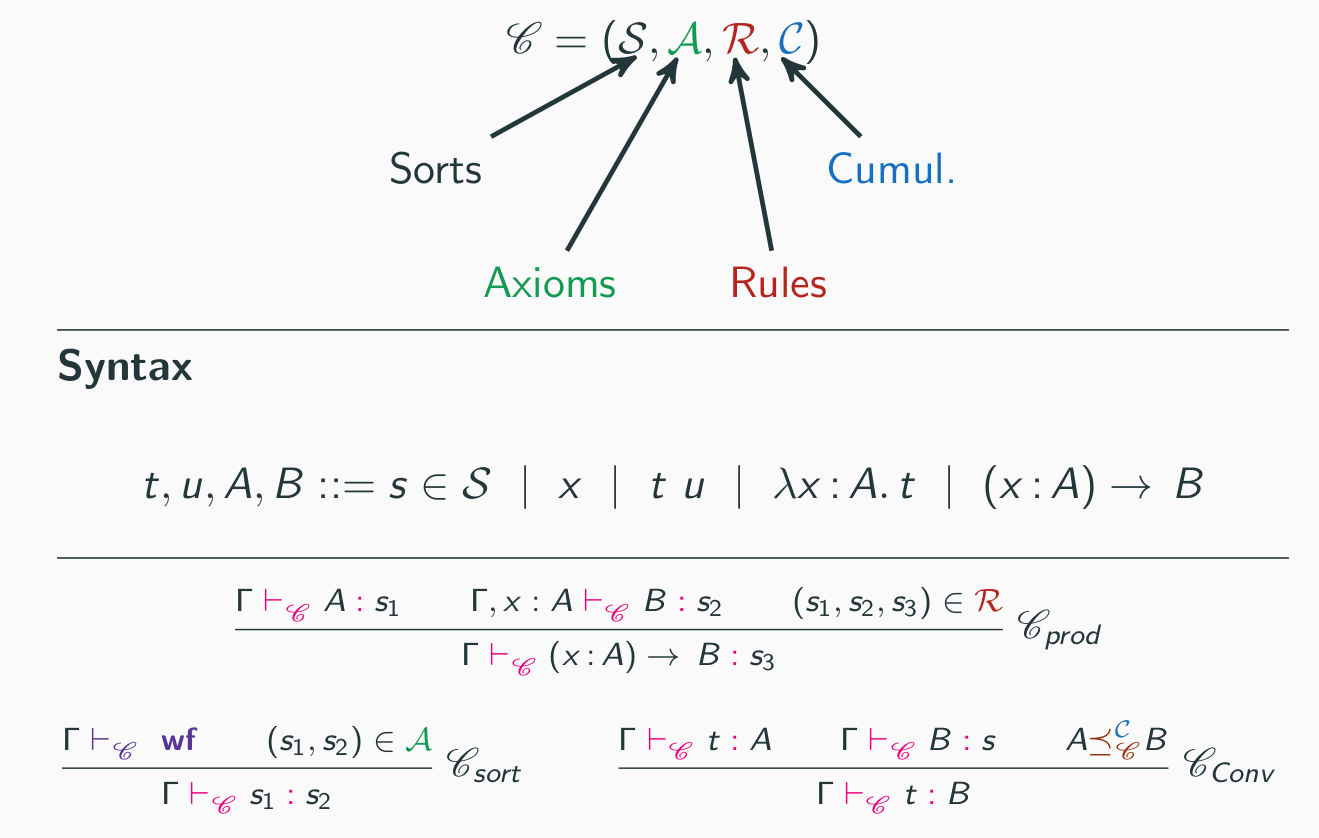
\includegraphics[scale=0.2]{images/cts.png}
  \end{center}    
\end{frame}

\begin{frame}{Graph representation of a CTS}
  \begin{center}    
    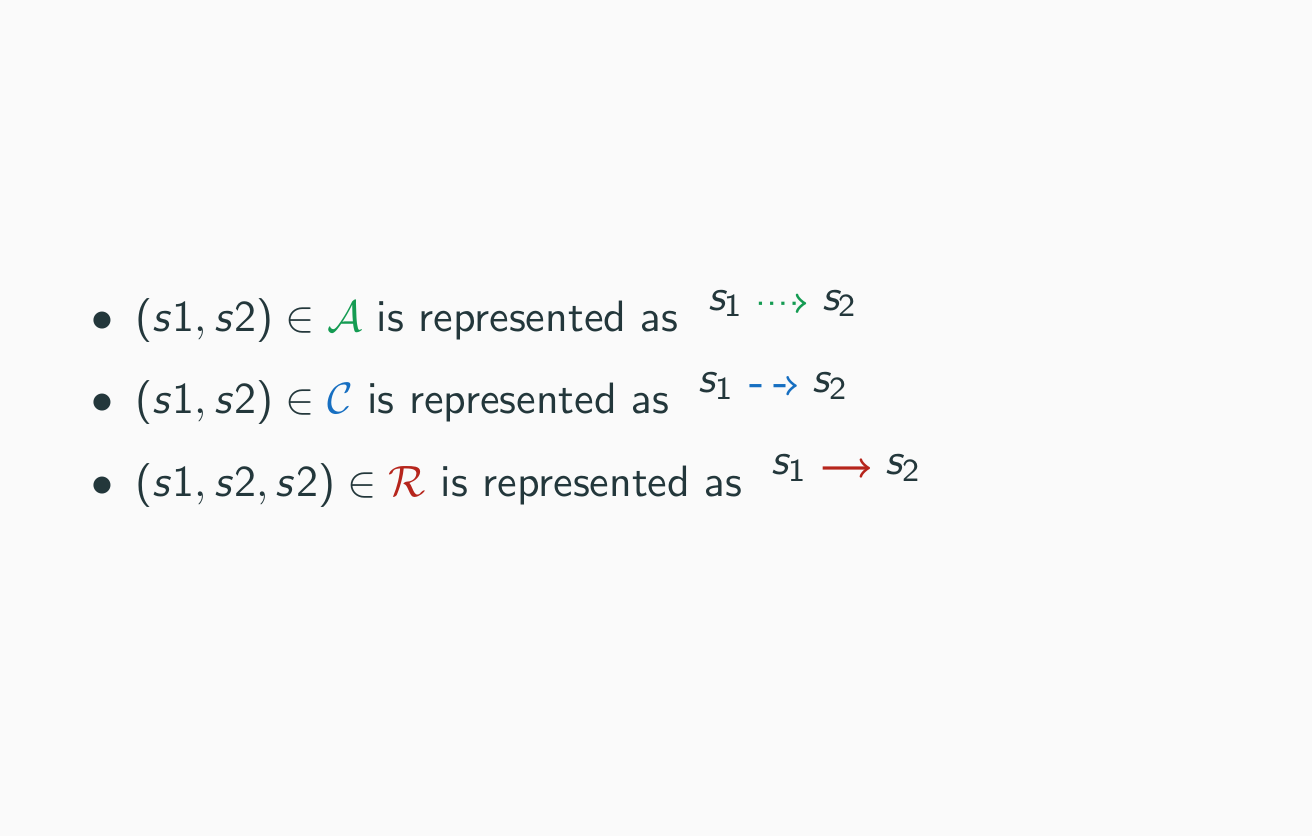
\includegraphics[scale=0.2]{images/graph.png}
  \end{center}    
\end{frame}

\begin{frame}{STT\(\forall\) as a CTS}
  \begin{center}    
    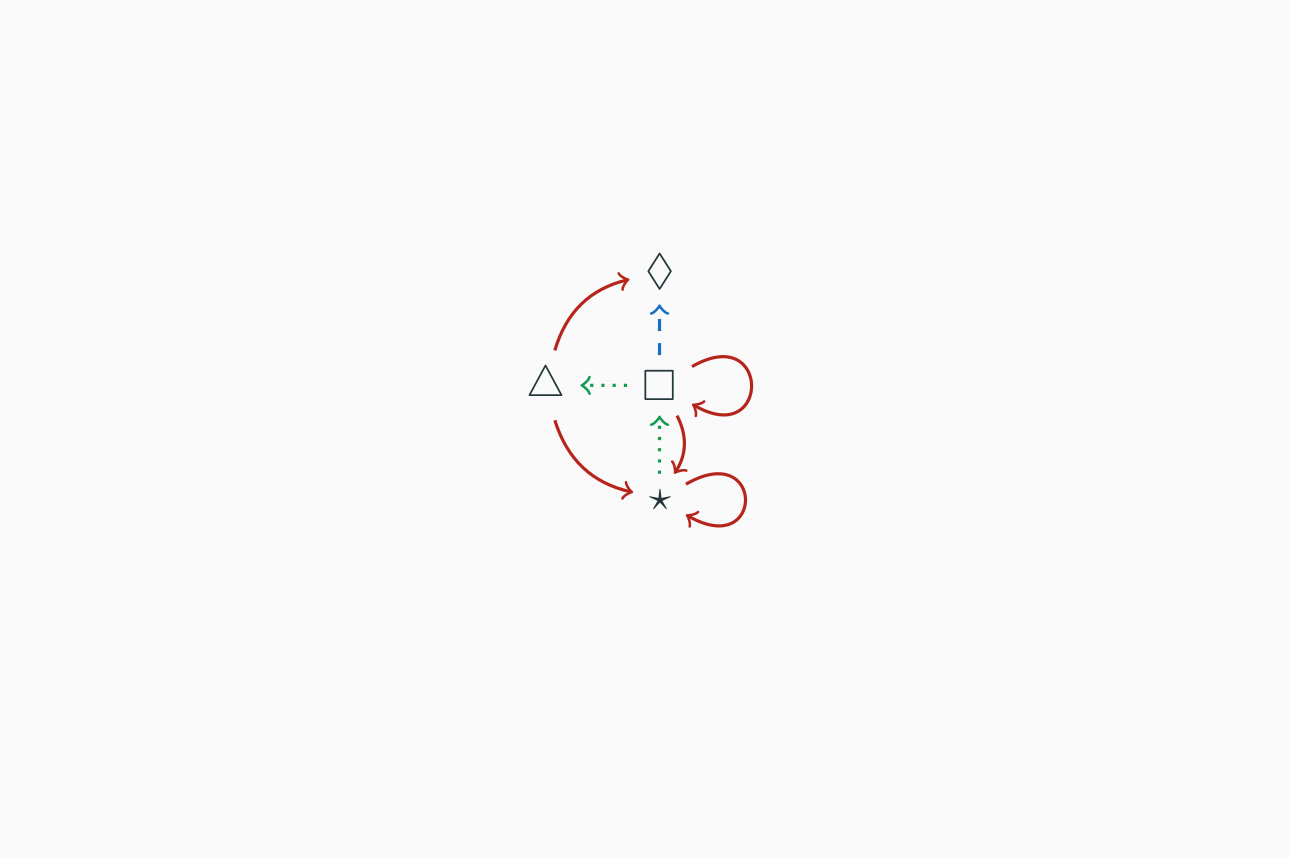
\includegraphics[scale=0.2]{images/sttfa_cts.png}
  \end{center}    
\end{frame}

\begin{frame}{Demo}
  \large{Let's use Dkmeta to go from the usual STT\(\forall\)
    representation to its CTS representation.}
\end{frame}

\section{Universo}

\begin{frame}{Remember}
  \begin{center}    
    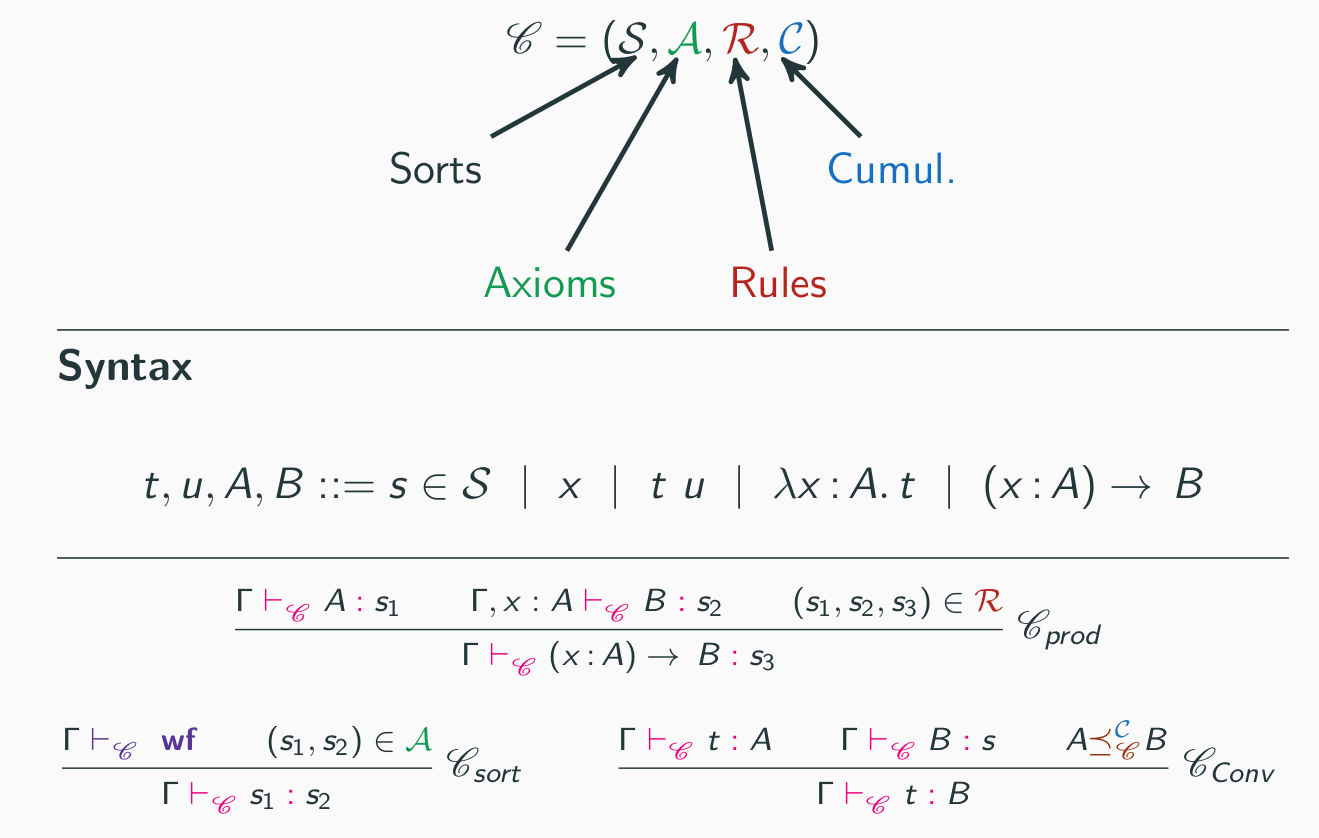
\includegraphics[scale=0.2]{images/cts.png}
  \end{center}    
\end{frame}

\begin{frame}
  \frametitle{Universo}

  \begin{itemize}
  \item \blue{Universo} is about 1000 lines of OCaml
  \item \orange{Independent} of the CTS specification
  \item Can be used to go from an \blue{impredcative theory} to a predicative
    one
  \item Can be used to encode \blue{floating universes} in Dedukti
  \item Can be used to \blue{minimize} the number of universes needed
  \item Can be used to know whether some \blue{proofs} can \blue{be encoded} into another!
  \end{itemize}
\end{frame}


\begin{frame}
  \only<1>{ \frametitle{Paradox in Type Theory} } \only<2->{
    \frametitle{Universes} } \framesubtitle{A solution to Girard's
    paradox}

  \only<1>{
    \[
      \Rule{\Gamma \vdash Type : Type}{} \text{ \xmark}
    \]
  } \only<2>{
    \begin{mathpar}
      \addrule{\Rule{\vdash U_{\un{i}} : U_{\un{i+1}}}{}}
      \addrule{\RulePP{\Gamma \vdash A : U_{\un{i}}}{\Gamma, x : A
          \vdash B : U_{\un{i}}}{\Gamma \vdash (x:A) \to B :
          U_{\un{i}}}{}}
    \end{mathpar}
  } \only<3-5>{
    \begin{mathpar}
      \addrule{\Rule{\vdash \transp{U_{\un{i}} : U_{\un{i+1}}}}{}}
      \addrule{\RulePP{\transp{\Gamma \vdash A :
            U_{\un{i}}}}{\transp{\Gamma, x : A \vdash B :
            U}_{\un{i}}}{\transp{\Gamma \vdash (x:A) \to B :
            U}_{\un{i}}}{}}
    \end{mathpar}
    \only<3>{
      \[\Prop \defn U_0\]
      \[\Type \defn U_1\]
      \[\Kind \defn U_2\]
    } \only<4-5>{
      \[nat : \Type\]
      \[ nat \to nat : \Type\]
      \[ \Type \to \Type : \Kind \]
      \[\top \to \top : \Prop\]
      \only<5>{
        \[(x : \Type) \to \top \text{ \xmark }\]
        \[nat \to \Type \text{ \xmark }\] } } } \only<6-9>{
    \begin{mathpar}
      % \addrule{\Rule{\vdash U_i~type}{}} \addrule{\RuleP{\Gamma
      % \vdash A : U_i~type}{\Gamma \vdash A~type}{}}
      \addrule{\Rule{\vdash \transp{U}_{\un{i}} :
          \transp{U}_{\un{i+1}}}{}} \addrule{\RulePP{\transp{\Gamma
            \vdash A :} U_{\un{i}}}{\transp{\Gamma, x : A \vdash B :}
          U_{\un{j}}}{\transp{\Gamma \vdash (x:A) \to B} :
          U_{\un{rule(i,j)}}}{}}
    \end{mathpar}
    \only<7-9>{
      \begin{align*}
        rule(i,0) &\defn 0 \text{ \transp{(impredicativity)}} \\
        rule(i,j+1) &\defn max(i, j + 1)
      \end{align*}

    } \only<8-9>{
      \[(x : \Type) \to \top : \Prop\]
      \[ (X : \Type) \to X \to X \to \Prop : \Kind\] } \only<9>{
      \[((x : \Type) \to x =_{\Type} x)~\top \text{ \xmark}\] } }
  \only<10-12>{
    \begin{mathpar}
      \addrule{\Rule{\vdash \transp{U}_{\un{i}} :
          \transp{U}_{\un{i+1}}}{}} \only<10>{
        \addrule{\RulePP{\transp{\Gamma \vdash A} :
            U_{\un{i}}}{\un{i\leq j}}{\transp{\Gamma \vdash A }:
            U_{\un{j}}}{}} } \only<11-12>{
        \addrule{\RuleP{\transp{\Gamma \vdash A} :
            U_{\un{i}}}{\transp{\Gamma
              \vdash}\textcolor{black}{\uparrow_{\un{i}}^{\un{j}}}
            \transp{A }: U_{\un{max~i~j}}}{}} }
      \addrule{\RulePP{\transp{\Gamma \vdash A :}
          U_{\un{i}}}{\transp{\Gamma, x : A \vdash B :}
          U_{\un{j}}}{\transp{\Gamma \vdash (x:A) \to B} :
          U_{\un{rule~i~j}}}{}}
    \end{mathpar}

    \only<12>{
      \[((x : \Type) \to x = x)~\uparrow_{\Prop}^{\Type} \top \text{
          \cmark}\]
      \[((x : \Type) \to x = x)~nat \text{ \cmark}\] } }
\end{frame}

\begin{frame}
  \frametitle{A minimization problem}

  \begin{center}
    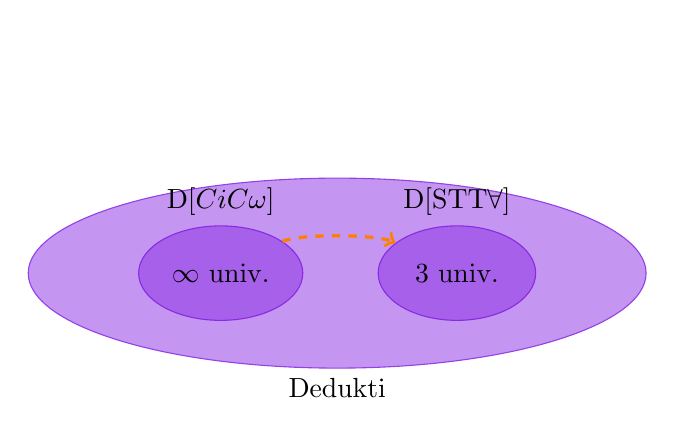
\begin{tikzpicture}
      [node distance=3cm, on grid, checker/.style = {shape=ellipse,
        draw=blue-violet!100, fill=blue-violet!25, align=center,
        minimum height=1.2cm, minimum width=2cm}, dedukti node/.style
      = {shape=ellipse, draw=blue-violet!90, fill=blue-violet!50,
        label={south:Dedukti}}, post/.style={->, >=stealth',
        semithick}]

      \node [checker, fill=blue-violet!75, label={north:D[\sttm{}]}]
      (DOT) {\(3\) univ.}; \node [checker, left=of DOT,
      fill=blue-violet!75, label={north:D[\cicw]}] (DMatita)
      {\(\infty\) univ.};
      \begin{scope}[on background layer]
        \node [dedukti node, inner sep=7pt, fit={(DMatita) (DOT)}]
        (Dedukti) {};
      \end{scope}
      \node [draw=none] (Coq) [above=of Dedukti] {}; .. controls
      ([yshift=-0cm,xshift=-3cm]Dedukti) .. (DMatita); .. controls
      ([yshift=-0cm,xshift=3cm]Dedukti) .. (DOT); .. controls
      ([yshift=-0cm,xshift=3cm]Dedukti) .. (DOT);

      \draw[very thick, orange, dashed, ->] (DMatita) .. controls
      ([xshift=-0.5cm,yshift=0.5cm]Dedukti) and
      ([xshift=0.5cm,yshift=0.5cm]Dedukti) .. (DOT);
    \end{tikzpicture}
  \end{center}
\end{frame}

\begin{frame}
  \frametitle{} \only<1>{
    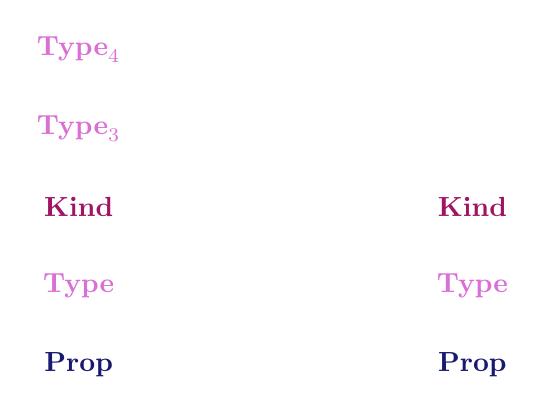
\begin{tikzpicture}
      \node at (0,10) {\Typefour}; \node at (0,9) {\Typethree}; \node
      at (0,8) {\Kind}; \node at (0,7) {\Type}; \node at (0,6)
      {\Prop}; \node at (5,8) {\Kind}; \node at (5,7) {\Type}; \node
      at (5,6) {\Prop};
    \end{tikzpicture}
  } \only<2>{
    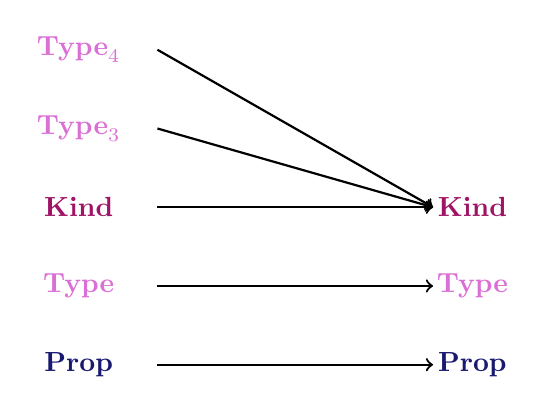
\begin{tikzpicture}
      \node at (0,10) {\Typefour}; \node at (0,9) {\Typethree}; \node
      at (0,8) {\Kind}; \node at (0,7) {\Type}; \node at (0,6)
      {\Prop}; \node at (5,8) {\Kind}; \node at (5,7) {\Type}; \node
      at (5,6) {\Prop}; \draw[thick,->] (1,10) -- (4.5,8);
      \draw[thick,->] (1,9) -- (4.5,8); \draw[thick,->] (1,8) --
      (4.5,8); \draw[thick,->] (1,7) -- (4.5,7); \draw[thick,->] (1,6)
      -- (4.5,6);
    \end{tikzpicture}
  } \only<3>{
    \begin{tikzpicture}
      \node at (0,10) {\Typefour}; \node at (0,9) {\Typethree}; \node
      at (0,8) {\Kind}; \node at (0,7) {\Type}; \node at (0,6)
      {\Prop}; \node at (5,8) {\Kind}; \node at (5,7) {\Type}; \node
      at (5,6) {\Prop}; \draw[thick,->] (1,10) -- (4.5,8);
      \draw[thick,->] (1,9) -- (4.5,8); \draw[thick,->, dashed] (1,8)
      -- (4.5,8); \draw[thick,->, dashed] (1,8) -- (4.5,8);
      \draw[thick,->, dashed] (1,8) -- (4.5,7); \draw[thick,->,
      dashed] (1,7) -- (4.5,7); \draw[thick,->, dashed] (1,7) --
      (4.5,6); \draw[thick,->] (1,6) -- (4.5,6); \node at (8,8)
      {\(\Rule{\vdash \transp{U}_{\un{i}} :
          \transp{U}_{\un{i+1}}}{}\)};
    \end{tikzpicture}
  }
\end{frame}

\begin{frame}
  \frametitle{Universo's algorithm}
  \begin{enumerate}
  \item Elaboration: \blue{Replace} every universe by a fresh variable
  \item Checking: Generate \blue{constraints} by type checking the
    terms (with an implementation of Dedukti)
  \item Resolution: \blue{Solve} the constraints (using an SMT solver)
  \item Reconstruction: \blue{Replace} the solution found for every terms
  \end{enumerate}
\end{frame}

\begin{frame}{Coq as a CTS}
  \begin{center}    
    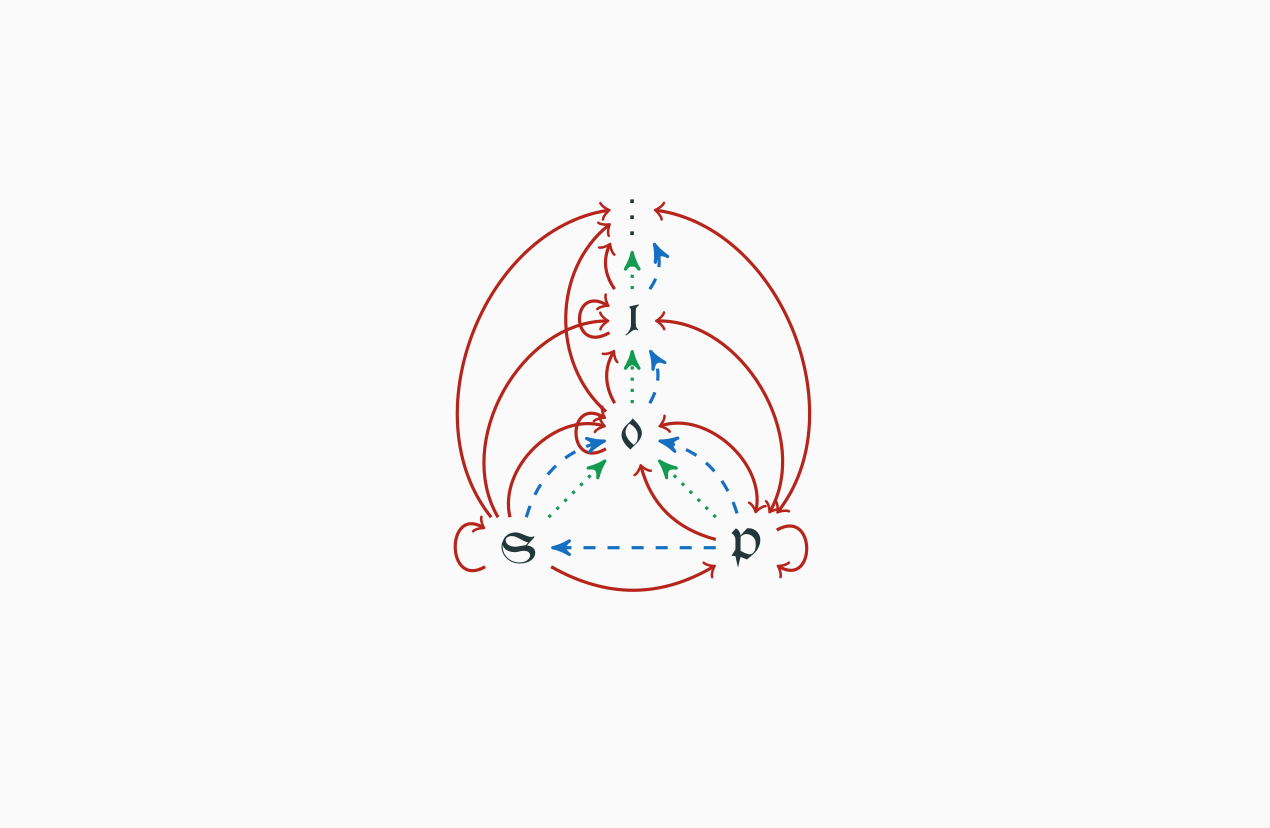
\includegraphics[scale=0.2]{images/coq_cts.png}
  \end{center}    
\end{frame}

\begin{frame}{Demo}
  \large{Let's use Universo to see whether the proofs using the
    STT\(\forall\) representation can translated into the Coq
    representation with \(3\) universes!}
\end{frame}

\section{Conclusion}

\begin{frame}
  \begin{block}{Question}
    \Large{What are the advantages of using Dedukti for \orange{interoperability}?}
  \end{block}
\end{frame}

\begin{frame}{Dedukti's advantages}
  \begin{itemize}
  \item Dedukti aims to be a \green{standard} to write logics
  \item Implementing this standard or \green{relevant part} of this
    standard is rather \green{easy}
  \item (Higher-Order) rewriting is a \green{powerful mechanism} to
    embed logics (encodings are small) and to \green{transform}
    Dedukti terms
  \item Dedukti's encodings \green{highlight common features} of
    several logics
  \item Dedukti's encodings allow to \green{better understand} the
    object logic (both practically and theoretically)
  \end{itemize}
\end{frame}

\begin{frame}{Features in Dedukti}

  Given a \blue{feature} of a logic (inductive
  types, universes, classical connectives, eta-reduction, ...):
  \begin{itemize}
  \item Their \orange{encoding} does not depend on the object logic
    (empirical fact)
  \item There might exist several \orange{variants} in Dedukti (which
    is a \green{good} property)
  \end{itemize}
\end{frame}

\begin{frame}{Main takeaway}
    \begin{center}
      \Large{\green{Scalability} of proof interoperability of proofs
        with \blue{Dedukti} depends on the ability to \orange{encode
          features separately} and to \orange{combine} them.}
  \end{center}
\end{frame}
\end{document}

%%% Local Variables: 
%%% TeX-command-extra-options: "-shell-escape"
%%% End:
